%%%%%%%%%%%%%%%%%%%%%%%%%%%%%%%%%%%%%%%%%%%%%%%%%%%%%%%%%%%%%%%
%
% Welcome to Overleaf --- just edit your LaTeX on the left,
% and we'll compile it for you on the right. If you open the
% 'Share' menu, you can invite other users to edit at the same
% time. See www.overleaf.com/learn for more info. Enjoy!
%
%%%%%%%%%%%%%%%%%%%%%%%%%%%%%%%%%%%%%%%%%%%%%%%%%%%%%%%%%%%%%%%


% Inbuilt themes in beamer
\documentclass{beamer}

% Theme choice:
\usetheme{CambridgeUS}

% Title page details: 
\title{Assignment 6} 
\author{Varun Gupta \\ cs21btech11060}
\date{\today}
\logo{\large \LaTeX{}}


\begin{document}

% Title page frame
\begin{frame}
    \titlepage
\end{frame}

% Remove logo from the next slides
\logo{}


% Outline frame
\begin{frame}{Outline}
    \tableofcontents
\end{frame}
\section{Class 12 Solutions}
\begin{frame}{Problem}
    \begin{block}{Example 30}
        Six balls are drawn successively from an urn containing 7 red and 9 black balls.Tell whether or not the trials of drawing ball are Bernoulli trials when after each draw the ball drawn is
        \begin{enumerate}
            \item replaced
            \item not replaced in the urn
        \end{enumerate}
    \end{block}
\end{frame}
\begin{frame}{Solution}
    \begin{block}{Solution:}
        \begin{enumerate}
            \item  The number of trials is finite. When the drawing is done with replacement, the
                  probability of success (say, red ball) is p = $\frac{7}{16}$ which is same for all six trials. Hence, the drawing of balls with replacements are Bernoulli trials.
            \item When the drawing is done without replacement, the probability of success in first trial is $\frac{7}{16}$, in 2nd trial is $\frac{6}{15}$ if the first ball drawn is red or $\frac{7}{15}$ if the first ball drawn is black and so on. Clearly, the probability of success is not same for all trials, hence the trials are not Bernoulli trials.
        \end{enumerate}
    \end{block}
\end{frame}
\begin{frame}{Code}
        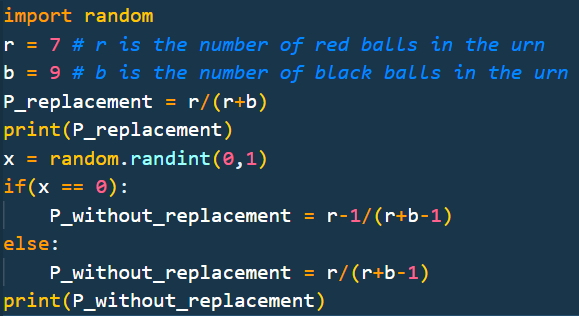
\includegraphics{figures/fig.png}
\end{frame}
\end{document}